\documentclass{article}

\makeatletter
\def\input@path{{../../docs/}}
\makeatother

\PassOptionsToPackage{numbers,compress}{natbib}
\usepackage[dblblindworkshop]{neurips_2026}
\workshoptitle{Foundation Models for the Brain and Body}

\usepackage[utf8]{inputenc}
\usepackage[T1]{fontenc}
\usepackage{hyperref}
\usepackage{url}
\usepackage{booktabs}
\usepackage{amsmath}
\usepackage{amsfonts}
\usepackage{microtype}
\usepackage{xcolor}
\usepackage{graphicx}
\usepackage{placeins}
\graphicspath{{../../docs/figures/}}
\hypersetup{hidelinks}

\title{From Public URLs to Honest Generalization: A Leakage-Aware Protocol for Continual Gait Representation Learning}
\author{Anonymous authors}

\begin{document}
\maketitle

\begin{abstract}
Public-video datasets make movement representation learning accessible, but they also create an evaluation problem: many annotated sequences can come from one upload, source availability changes, the same person may cross uploads, and pose-estimation failures can correlate with dataset labels. We use a project-specific, S-JEPA-inspired gait pipeline as a case study and specify a leakage-aware protocol for continual movement representation learning. A September 4, 2026 audit retained 657 of 666 annotated sequences at the metadata gate, 655 at the decoded-span gate, and 639 from 97 source videos after pose QC. The protocol partitions sources before fitting, trains the encoder only on outer-training sources, reserves grouped validation sources for selection, and opens grouped test sources only for final evaluation. Label-free JEPA plus VICReg is primary; a label-aware condition loss is a supervised ablation. One fully traced fold-and-seed execution verifies the mechanics and exposes an important negative result: a raw-kinematic readout outperformed the learned latent readout on 20 held-out sources. We report this as a worked execution, not a cross-fold or clinical estimate. The contribution is an auditable evaluation design and evidence discipline for behavioral foundation-model research.
\end{abstract}

\section{Introduction}

Pose extracted from video is a behavioral signal at the interface of body dynamics, environment, and sensing. It is therefore a useful modality for studying self-supervised and continually adapted representations. It is also unusually vulnerable to false generalization: excerpts from the same upload share camera, compression, demonstrator, background, and pose-estimator behavior. A random sequence split can place these signatures on both sides of evaluation.

We study these issues through a normal-first skeleton JEPA case study. The implementation is inspired by S-JEPA but is not a reproduction of it: it uses a fixed 12-landmark target whitelist and auxiliary VICReg, with an optional label-aware group objective. Rather than promote a stale score, we ask what evidence would justify three distinct claims: that a representation retains normal-gait information during adaptation, that its features support a downstream readout, and that performance transfers to unseen sources.

Our contributions are: (1) a dated, status-defined census of a changing public-video corpus; (2) a source-grouped train/validation/test protocol that encloses preprocessing, encoder training, and readout fitting; (3) a separation between label-free representation learning and label-informed ablation; and (4) a claim and ethics ledger for public gait video. The case study directly connects BrainBodyFM themes of pose and movement, self-supervised and continual learning, evaluation, generalization, and reproducibility. It does not claim that this small model or corpus is itself foundation-scale.

\section{Related work}

JEPAs predict target-encoder features rather than reconstructing each input value. I-JEPA applies the idea to images \citep{assran2023ijepa}, V-JEPA to video \citep{bardes2024vjepa}, and S-JEPA to skeleton sequences \citep{abdelfattah2024sjepa}. VICReg supplies invariance, variance, and covariance regularization \citep{bardes2022vicreg}. Markerless pose makes gait analysis scalable, but it also introduces viewpoint, visibility, and detector-dependent errors \citep{grishchenko2022blazepose,mediapipePoseLandmarker}. When observations share a source, validation must respect that grouping \citep{roberts2017crossvalidation}. Our focus is the complete evaluation boundary around a continually updated representation, rather than a new clinical classifier.

\section{Case-study data boundary}

\subsection{Annotations and live metadata census}

GAVD provides annotations and public video identifiers for five folder categories: normal, Parkinson's, stroke, myopathic, and cerebral palsy \citep{ranjan2025gavd}. These are dataset annotations, not diagnoses made by this project. The local five-part inventory contains 666 sequence files from 103 source videos.

We performed a fresh public-metadata check on September 4, 2026. Three sources did not expose public metadata: \texttt{sf5X4YYkWUA} and \texttt{YjRoLtP1di0} were private, and \texttt{yULxvDc9e8c} was unavailable. Table~\ref{tab:census} reports the resulting snapshot.

\begin{table}[htbp]
\caption{Annotated inventory and September 4, 2026 public-metadata census. Counts are sequences / source videos.}
\label{tab:census}
\centering
\small
\begin{tabular}{lrr}
\toprule
Folder annotation & Raw inventory & Metadata-public \\
\midrule
Normal & 291 / 32 & 291 / 32 \\
Parkinson's & 47 / 11 & 47 / 11 \\
Stroke & 76 / 19 & 75 / 18 \\
Myopathic & 188 / 30 & 184 / 29 \\
Cerebral palsy & 64 / 11 & 60 / 10 \\
\midrule
Total & 666 / 103 & 657 / 100 \\
\bottomrule
\end{tabular}
\end{table}

\begin{figure}[t]
  \centering
  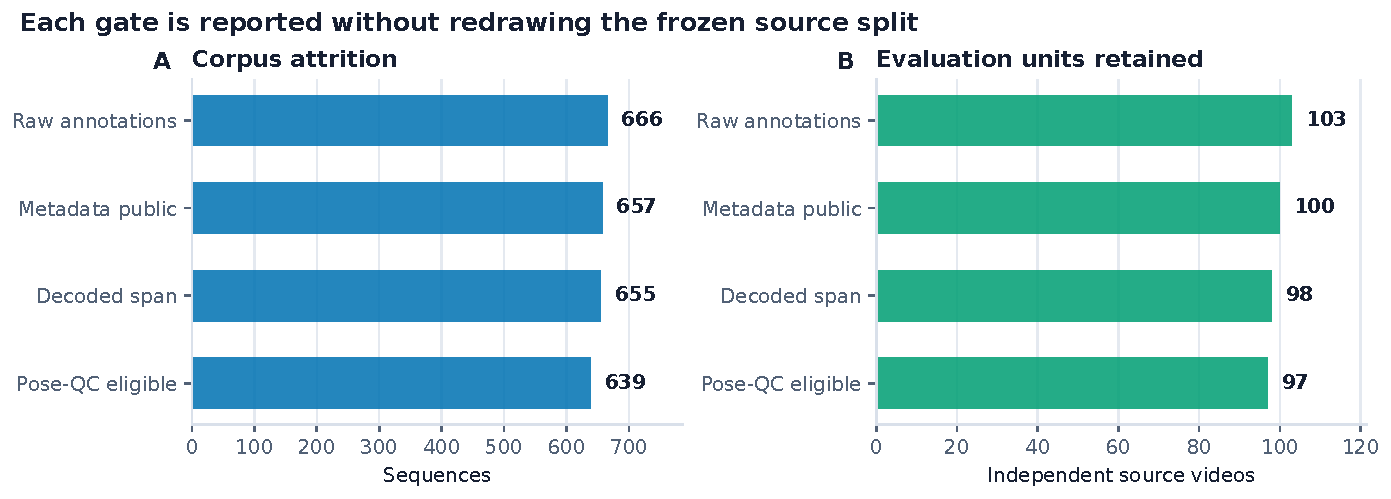
\includegraphics[width=0.98\linewidth]{bbfm_data_funnel.pdf}
  \caption{Dated corpus attrition at both sequence and source-video scales. The split is frozen before decode and pose-QC attrition, so later failures remove observations without changing any source's role.}
  \label{fig:data-funnel}
\end{figure}

``Metadata-public'' has a deliberately narrow meaning: the service returned current metadata without authentication during this audit. It does not prove that an appropriate media format can be downloaded, that the file reaches every annotated frame, that decoding succeeds, or that pose coverage is adequate. Those are later gates and must be reported separately. Availability also varies with time, region, account state, and platform behavior; every paper census therefore needs a timestamp, status vocabulary, tool version, and immutable audit artifact.

\subsection{Pose and model case study}

The pipeline extracts 33 MediaPipe landmarks and visibility values, interpolates short internal gaps, pelvis-centers and body-scale normalizes coordinates, and resizes each segment to 64 frames. A token represents one landmark over four frames. Only valid tokens from shoulders, hips, knees, ankles, heels, and foot tips may become prediction targets.

The case-study model contains a view encoder, an exponential-moving-average target encoder, and a predictor. The proposed primary objective is label-free:
\begin{equation}
\mathcal L_{\mathrm{primary}}=\mathcal L_{\mathrm{JEPA}}+0.05\mathcal L_{\mathrm{VICReg}}.
\end{equation}
The historical pipeline also used a condition-label group term after normal-only training. Because that term directly encourages within-label compactness and between-label separation, it belongs in a supervised ablation,
\begin{equation}
\mathcal L_{\mathrm{ablation}}=\mathcal L_{\mathrm{primary}}+0.25\mathcal L_{\mathrm{group}},
\end{equation}
not in the primary self-supervised claim. This distinction prevents downstream label readability from being presented as independently discovered structure.

\section{Leakage-aware evaluation protocol}

\subsection{Split before fitting}

The independent unit is the source-video ID, not a sequence row. We first canonicalize video identifiers, attach the dated availability status, and assign every source to exactly one outer fold. Splits are approximately stratified by folder annotation while balancing both source and sequence counts; the complete source lists and a split-manifest digest are frozen before model fitting. Because the smallest categories contain only ten or eleven metadata-public sources, a single holdout is unstable. The primary estimate should use repeated, source-grouped outer splits or stratified grouped cross-validation and expose that sensitivity rather than hide it.

\begin{figure}[t]
  \centering
  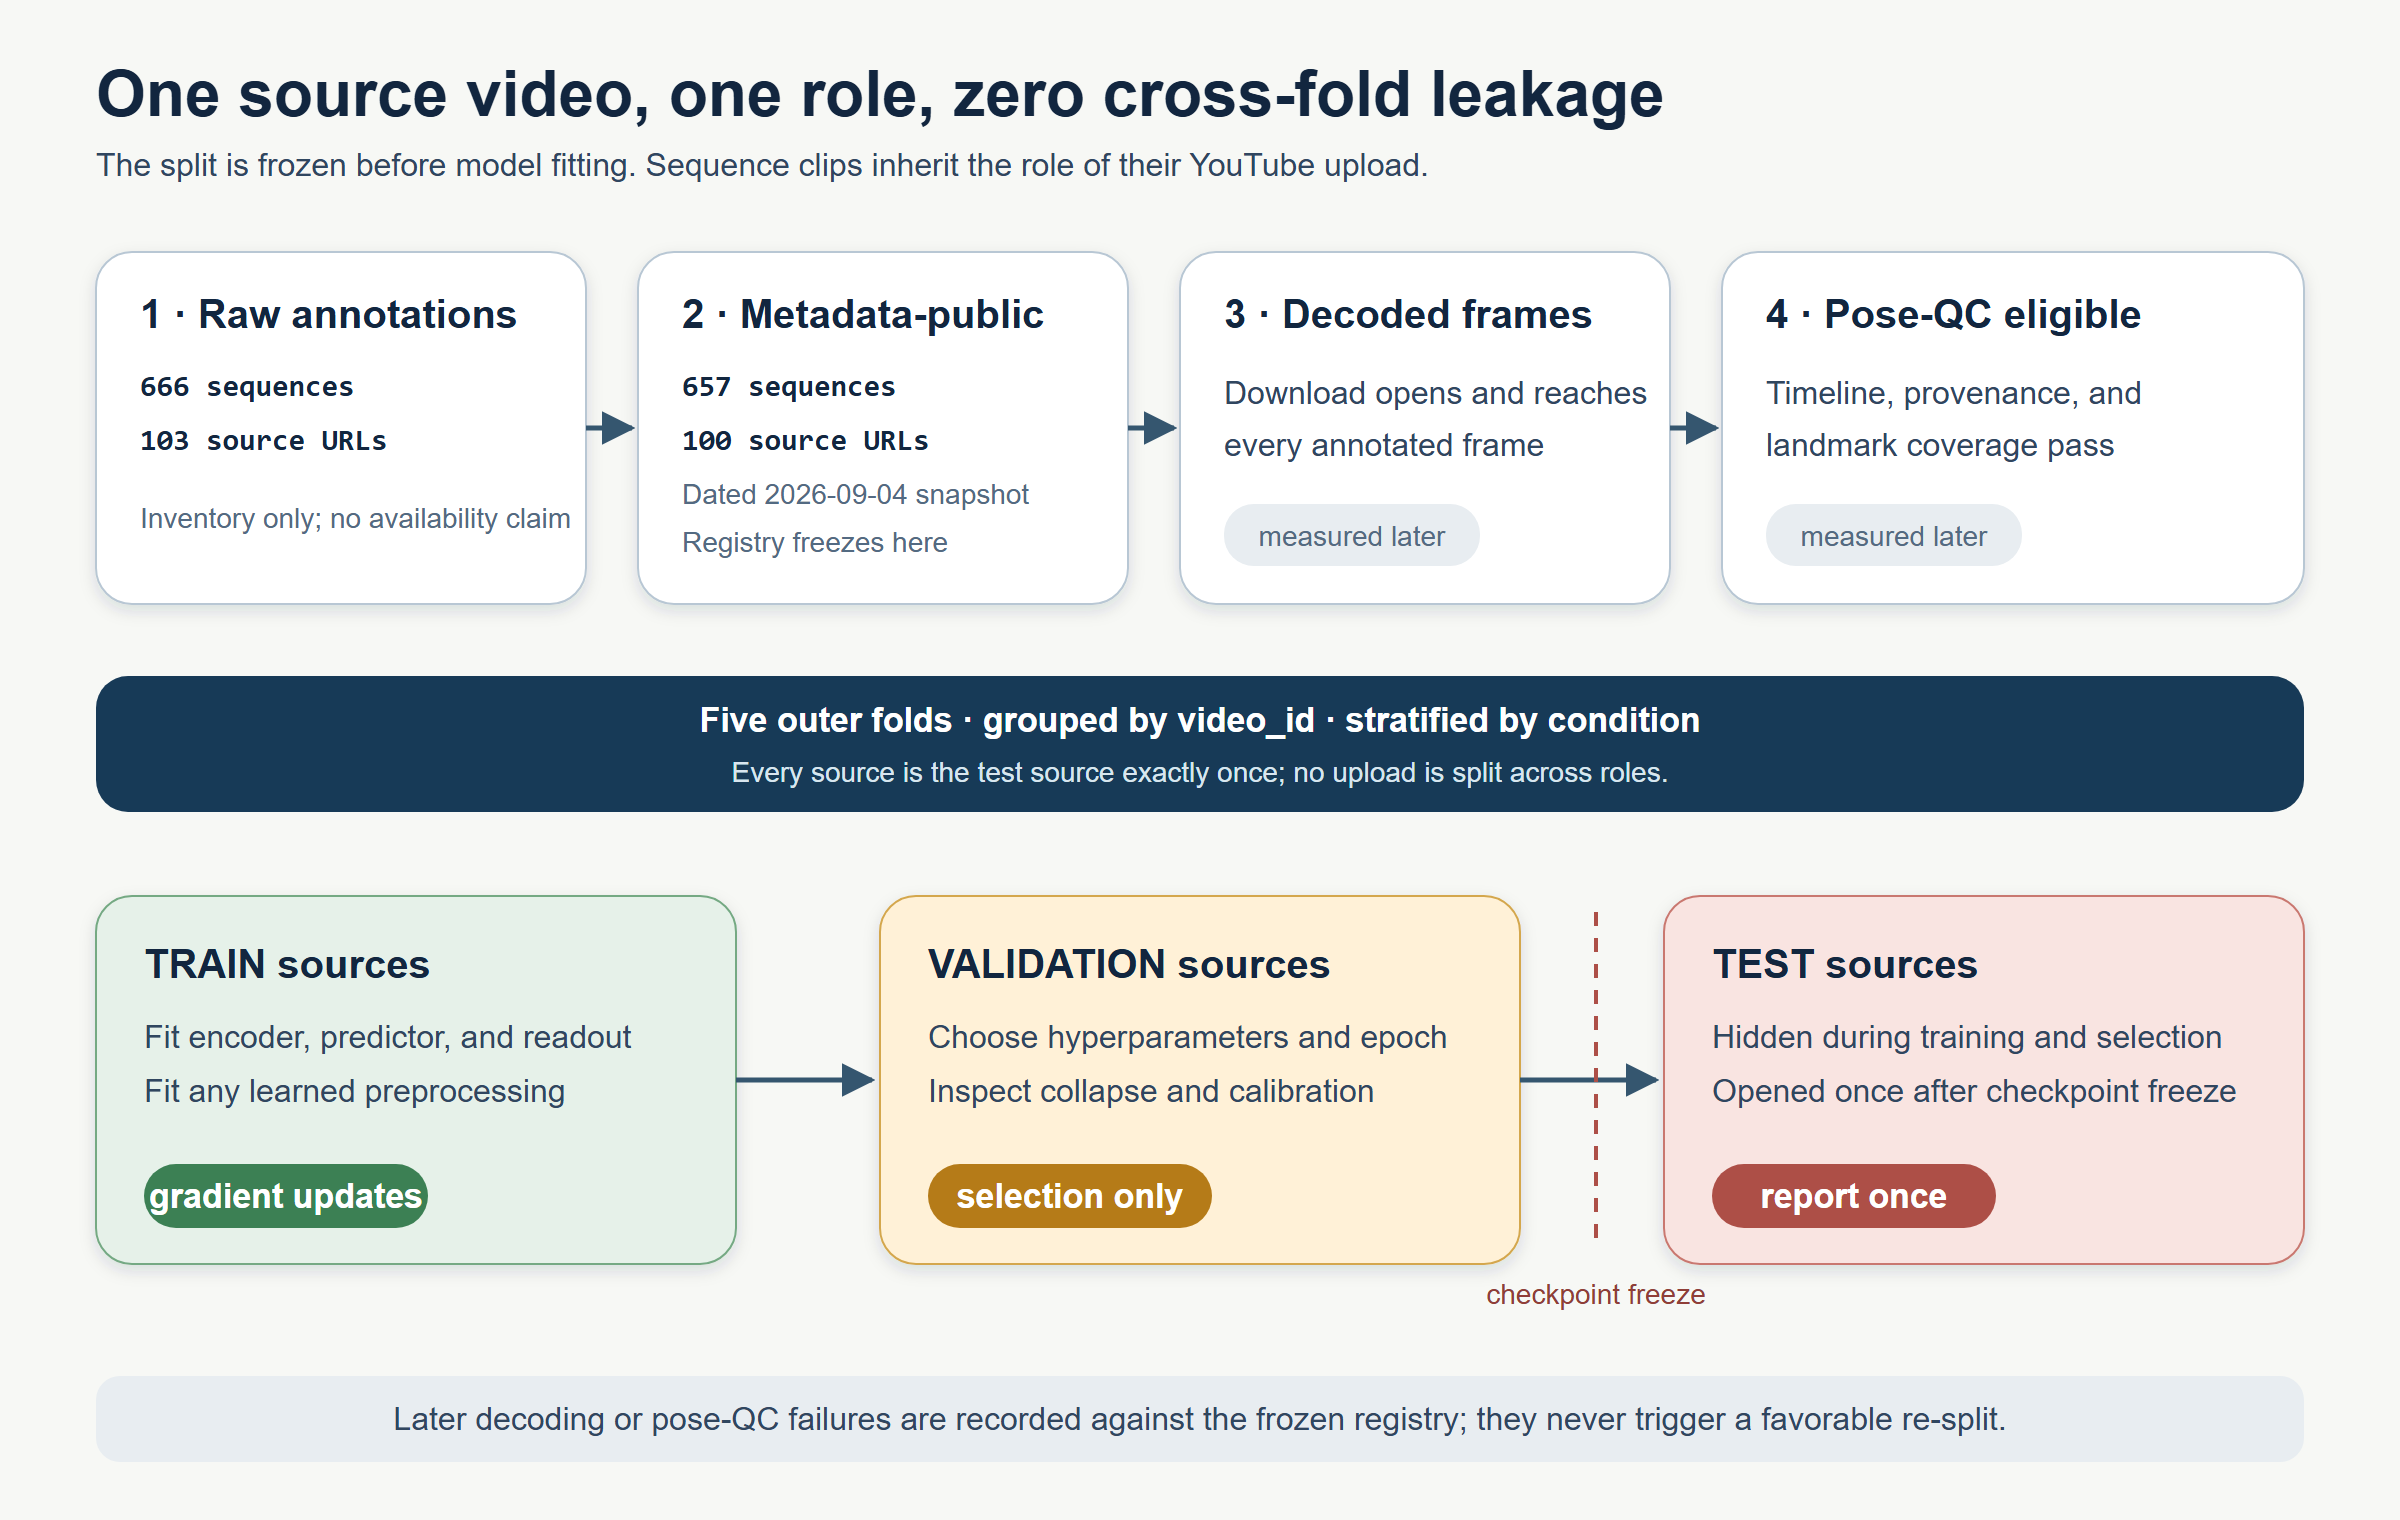
\includegraphics[width=0.98\linewidth]{inductive_source_split.png}
  \caption{The split freezes at the metadata-public gate. Every clip inherits its source video's role; later decode or pose-QC attrition is recorded without redrawing folds. Within an outer fold, only training sources receive gradient updates, validation sources select the checkpoint, and test sources remain sealed.}
  \label{fig:source-split}
\end{figure}

Inside each outer split, only training-source data may determine data-dependent preprocessing, quality thresholds, augmentation choices, model weights, or readout parameters. Grouped validation sources select hyperparameters, stopping rules, and checkpoints. The test sources remain sealed until the analysis is frozen. The full normal-first curriculum is retrained inside every outer training fold and for every seed. A source-grouped classifier on embeddings from an encoder trained on all sources is still transductive and is not a generalization estimate.

\subsection{Four endpoints, four claims}

We pre-specify four endpoints. First, training-source anchor curves are optimization telemetry. Second, retention is measured on held-out normal sources at each checkpoint using equal-source weighting, source-cluster uncertainty, alignment-aware comparisons such as orthogonal Procrustes and linear CKA, and a functional JEPA or perturbation-ranking task. Third, downstream readability fits a readout only on outer-training embeddings and reports balanced accuracy and macro-F1 on outer-test sources. Fourth, source transfer aggregates predictions by source and summarizes variability across outer splits and training seeds. None of these endpoints establishes person-level or clinical generalization.

The minimum comparison set is an untrained encoder, raw pose features, pose-validity or missingness features, continued-normal training with matched updates, and joint training. The label-aware group-loss arm is reported separately. Condition order is varied across seeds or included as a sensitivity analysis. All exclusions and failed runs remain in the ledger.

\FloatBarrier
\section{Worked protocol execution}

We executed outer fold 0 with seed 42 to test the complete artifact and isolation contract. Pose QC left 377 sequences from 59 training sources, 131 from 18 validation sources, and 131 from 20 test sources. Encoder fitting loaded only training tensors; checkpoint selection used validation loss; the serialized checkpoint records that test tensors were not opened. The five curriculum stages used 20 epochs each and saved a hash-bound checkpoint plus stage lineage.

After selection was frozen, source-level readouts were evaluated once on the 20 test sources (Fig.~\ref{fig:execution}). Macro-F1 was 0.292 for the S-JEPA latent, 0.251 for a missingness-only control, and 0.441 for raw kinematics. Thus this small learned representation did not beat the direct sensor-derived baseline in the worked fold. Normal-anchor cosine fell to 0.701 on five validation-normal sources after the full curriculum and was 0.850 on seven test-normal sources. Temporal probes retained some peak-phase and energy-ratio information but produced negative $R^2$ for phase lag. These results validate the protocol implementation and comparison set; with one fold and seed they do not estimate expected generalization.

\begin{figure}[t]
  \centering
  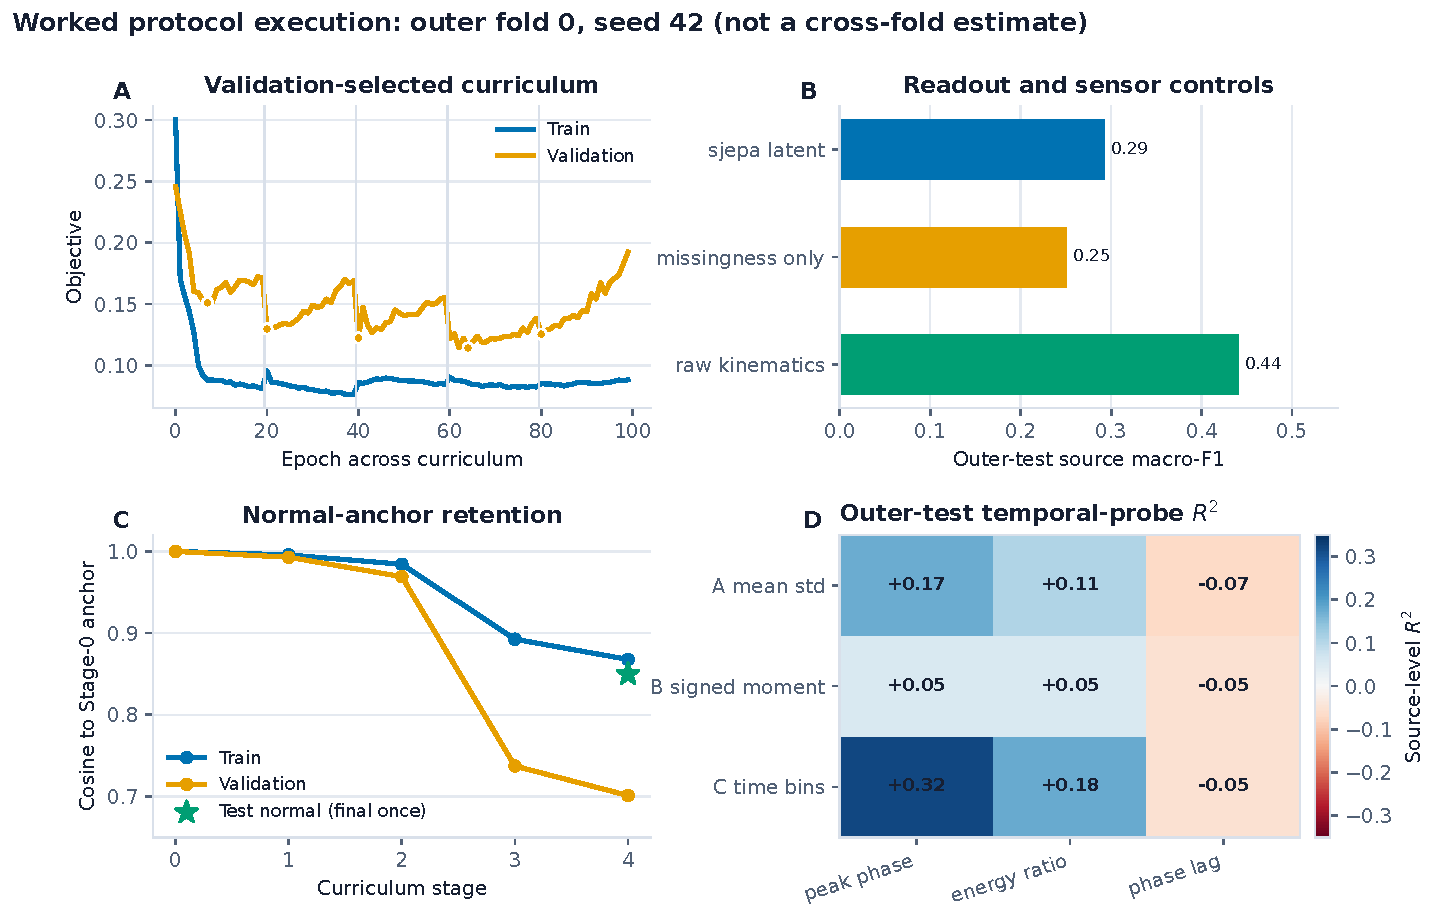
\includegraphics[width=0.98\linewidth]{bbfm_protocol_execution.pdf}
  \caption{Worked protocol-v2 execution (outer fold 0, seed 42). (A) Validation selects within each curriculum stage. (B) The raw-kinematic control exceeds the latent and missingness readouts on held-out sources. (C) Normal-anchor retention is selected on validation sources before one test-normal evaluation. (D) Temporal-probe results retain negative values. This is an execution audit, not a cross-fold estimate.}
  \label{fig:execution}
\end{figure}

Historical artifacts from the earlier sequence-level pipeline remain archived, not pooled with these values: those splits allowed source overlap, exposed evaluation rows to representation learning, and sometimes used folder labels during encoder training. A primary performance claim still requires all outer folds, multiple seeds, source-cluster uncertainty, and condition-order sensitivity.

\section{Limitations, data use, and ethics}

Source-video grouping is only the strongest available grouping key. GAVD does not provide a reliable person identifier for this analysis, so the same person may still cross folds through different uploads. Folder labels are not independently adjudicated here. Camera, compression, framing, clothing, mobility aids, demographic representation, editing, and pose-estimator visibility may correlate with labels. A source-held-out result must therefore be named as such, never subject-held-out or clinical performance.

Public availability is not equivalent to research consent or unrestricted reuse. GAVD distributes annotations and URLs rather than raw video, and places independent retrieval, platform compliance, institutional ethics approval, copyright, privacy, and data-protection obligations on users \citep{gavdRepo2026}. Gait and derived skeleton trajectories can be identifying even when faces are absent. Public artifacts should contain neither raw videos nor identity-bearing frames, and access to derived trajectories should be risk assessed. The project should record an ethics determination, data retention and access controls, and a takedown procedure before release. Language and analyses must avoid stigmatizing disability or presenting observational folder labels as diagnoses. No result in this case study supports diagnosis, treatment, surveillance, or deployment.

\section{Conclusion}

Behavioral foundation-model evaluation begins before training: with a dated source census, an explicit unit of independence, and a sealed evaluation path. In this public-video gait case study, nine annotated sequences lost public metadata when three of 103 source videos became private or unavailable. More importantly, metadata visibility is only the first of several data-validity gates. The proposed protocol keeps source videos disjoint throughout preprocessing, encoder learning, model selection, and downstream evaluation; separates label-free training from supervised ablation; and distinguishes retention, readability, source transfer, and clinical validity. One traced fold demonstrates that this discipline changes the scientific conclusion: the raw-kinematic baseline, not the learned latent, was strongest. Multi-fold performance remains pending.

\clearpage
\appendix

\section{Required run manifest}

Each reported run should record: source-manifest and availability-audit hashes; audit time, status definitions, and tool versions; decoded-frame and pose-quality decisions; source-level outer and validation split IDs; preprocessing configuration; label-use declaration; model and optimizer configuration; seed, condition order, hardware, and deterministic settings; parent and checkpoint hashes; exclusion reasons; and source-level predictions. Paper tables and figures should be generated from this manifest rather than copied manually.

\section{Claim ledger}

\begin{table}[h]
\centering
\small
\begin{tabular}{p{0.30\linewidth}p{0.29\linewidth}p{0.31\linewidth}}
\toprule
Claim & Required evidence & Current status \\
\midrule
Current metadata census & Dated per-source audit & Supported \\
Decoded/pose-usable cohort & Frame and pose gates & Supported by dated audit \\
Normal-function retention & Held-out normal sources & One fold/seed; exploratory \\
Unseen-source performance & Fold-local full retraining & One fold/seed; incomplete \\
Unseen-person performance & Reliable person groups & Not identifiable \\
Clinical validity & External adjudicated cohort & Not studied \\
\bottomrule
\end{tabular}
\end{table}

\bibliographystyle{plainnat}
\bibliography{../../docs/references}

\end{document}
